\documentclass[12pt,]{article}
\usepackage{lmodern}
\usepackage{amssymb,amsmath}
\usepackage{ifxetex,ifluatex}
\usepackage{fixltx2e} % provides \textsubscript
\ifnum 0\ifxetex 1\fi\ifluatex 1\fi=0 % if pdftex
  \usepackage[T1]{fontenc}
  \usepackage[utf8]{inputenc}
\else % if luatex or xelatex
  \ifxetex
    \usepackage{mathspec}
  \else
    \usepackage{fontspec}
  \fi
  \defaultfontfeatures{Ligatures=TeX,Scale=MatchLowercase}
\fi
% use upquote if available, for straight quotes in verbatim environments
\IfFileExists{upquote.sty}{\usepackage{upquote}}{}
% use microtype if available
\IfFileExists{microtype.sty}{%
\usepackage{microtype}
\UseMicrotypeSet[protrusion]{basicmath} % disable protrusion for tt fonts
}{}
\usepackage[margin=1in]{geometry}
\usepackage{hyperref}
\hypersetup{unicode=true,
            pdfborder={0 0 0},
            breaklinks=true}
\urlstyle{same}  % don't use monospace font for urls
\usepackage{longtable,booktabs}
\usepackage{graphicx,grffile}
\makeatletter
\def\maxwidth{\ifdim\Gin@nat@width>\linewidth\linewidth\else\Gin@nat@width\fi}
\def\maxheight{\ifdim\Gin@nat@height>\textheight\textheight\else\Gin@nat@height\fi}
\makeatother
% Scale images if necessary, so that they will not overflow the page
% margins by default, and it is still possible to overwrite the defaults
% using explicit options in \includegraphics[width, height, ...]{}
\setkeys{Gin}{width=\maxwidth,height=\maxheight,keepaspectratio}
\IfFileExists{parskip.sty}{%
\usepackage{parskip}
}{% else
\setlength{\parindent}{0pt}
\setlength{\parskip}{6pt plus 2pt minus 1pt}
}
\setlength{\emergencystretch}{3em}  % prevent overfull lines
\providecommand{\tightlist}{%
  \setlength{\itemsep}{0pt}\setlength{\parskip}{0pt}}
\setcounter{secnumdepth}{0}
% Redefines (sub)paragraphs to behave more like sections
\ifx\paragraph\undefined\else
\let\oldparagraph\paragraph
\renewcommand{\paragraph}[1]{\oldparagraph{#1}\mbox{}}
\fi
\ifx\subparagraph\undefined\else
\let\oldsubparagraph\subparagraph
\renewcommand{\subparagraph}[1]{\oldsubparagraph{#1}\mbox{}}
\fi

%%% Use protect on footnotes to avoid problems with footnotes in titles
\let\rmarkdownfootnote\footnote%
\def\footnote{\protect\rmarkdownfootnote}

%%% Change title format to be more compact
\usepackage{titling}

% Create subtitle command for use in maketitle
\newcommand{\subtitle}[1]{
  \posttitle{
    \begin{center}\large#1\end{center}
    }
}

\setlength{\droptitle}{-2em}
  \title{\Large{Biometry of the invasive lionfish (\textit{Pterois volitans}) in the Central Mexican Caribbean, and a review of allometric growth parameters across the invasion range}}
  \pretitle{\vspace{\droptitle}\centering\huge}
  \posttitle{\par}
\subtitle{\textbf{Running title}: Allometric growth of Pterois volitans}
  \author{}
  \preauthor{}\postauthor{}
  \date{}
  \predate{}\postdate{}

\usepackage{booktabs}
\usepackage{longtable}
\usepackage{array}
\usepackage{multirow}
\usepackage[table]{xcolor}
\usepackage{wrapfig}
\usepackage{setspace}
\doublespacing
\usepackage{lineno}
\linenumbers

\begin{document}
\maketitle

Juan Carlos VILLASEÑOR-DERBEZ\textsuperscript{1}

\textsuperscript{1} Bren School of Environmental Sciences and
Management, University of California Santa Barbara, Santa Barbara,
California, U.S.

* Correspondence: Juan Carlos Villaseñor-Derbez, Bren Hall, University
of California at Santa Barbara, Santa Barbara, CA, 93106, US phone: +1
207 205 8435, e-mail:
\href{mailto:jvillasenor@bren.ucsb.edu}{\nolinkurl{jvillasenor@bren.ucsb.edu}}

\clearpage

\textbf{Background.} Lionfish (\emph{Pterois volitans/miles}) are an
invasive species in the North-Western Atlantic and the Caribbean. In
order to better manage the invasion, inform lionfish removal programs,
predict their possible impacts, and estimate biomass available for
harvest, we must be able to accurately estimate their total biomass.
Previous work has identified that lionfish age-at-length relationships
are spatially variable across the invasion range. This work had two main
objectives: i) compare length-weight relationships of the invasive
lionfish through the invasion range; and ii) Report the length-weight
frequency for lionfish in the Central Meixcan Caribbean.

\textbf{Materials and methods.} A total of 13 length-weight
relationships reported in eight peer-reviewed studies and FishBase were
used to calculate expected biomass of organisms (n = 109) sampled from
the Central Mexican Caribbean, whose Total Length (TL) and Total Weight
(TW) were known. For each length-weight relationship,
expected-to-observed weight ratio was calculated for each organism.
Differences in mean expected-to-observed weight ratios were tested with
a one-way ANOVA; Tukey's HSD was used as a post-hoc test to identify
groups of non-statistically significant differences. Additionally, the
length-weight relationship of the 109 organisms was calculated. Total
Length (TL) and Total weight (TW) were log10-transformed to fit a linear
model describing the linearized length-weight relationship. The model
was fit using Ordinary Least Squares and Heteroskedastik-robust standard
errors were computed.

\textbf{Results.} Expected-to-observed weight ratios ranged from 0.44 to
3.51, and dfferences in weight-at-length were spatially consistent. For
a given length, parameters from the Caribbean yielded lower weights than
those from the Gulf of Mexico and Atlantic, indicating that
weight-at-length is spatially variable. This study also reports a new
pair of length-weight parameters
(\(a = 3.2056\times 10^{-6}; b = 3.235\)) for organisms sampled in the
Central Mexican Caribbean.

\textbf{Conclusion.} The large differences between observed and expected
biomass when using parameters from other locations highlights the
importance of using site-specific parameters to estimate biomass from
length observations. Findings from this work can aid managers and
decision makers to better select length-weight parameters when these are
not available for their region of interest.

\textbf{Key words}\\
lionfish, Pterois volitans, length-weight relationship, allometric
growth, Mexico

\clearpage

\section{INTRODUCTION}\label{introduction}

At least 84\% of the marine eco-regions have reported the presence of an
invasive species (Molnar et al., 2008). These represent a major threat
to local biodiversity and the economic activities that depend on it,
like tourism or fisheries (Bax et al., 2003). Invasive species may also
threaten native species through competition (DAVIS, 2003) or predation.
By 2005, the economic cost of invasive species to the United States was
estimated at \$120 billion per year and nearly 42\% of species that have
been included in the Endangered or Threatened species list have been
labeled as such due to presence of invasive species (Pimentel, Zuniga \&
Morrison, 2005). This highlights the importance of understanding,
managing, and preventing ecological invasions.

Lionfish (\emph{Pterois volitans/miles} complex) are an invasive species
in the North-Western Atlantic and the Caribbean, likely introduced
through liberation of aquarium-kept organisms (Betancur-R et al., 2011).
They are the first marine vertebrates to establish in North Atlantic
(Schofield, 2009, 2010) and Caribbean coasts (Sabido-Itza et al., 2016).
Lionfish have been widely reported in coral reefs (Aguilar-Perera \&
Tuz-Sulub, 2010), but also in other habitats such as estuaries (Jud et
al., 2011), mangroves (Barbour et al., 2010), areas with hard-bottoms
(Muñoz, Currin \& Whitfield, 2011), and mesophotic reefs (Andradi-Brown
et al., 2017). Due to its threat to local biodiversity, the speed of
their spread, and its difficulty of management, their presence in these
waters has been labeled as a major marine invasion (Hixon et al., 2016).

A significant amount of research has been done to describe lionfish
feeding ecology in North Carolina (Muñoz, Currin \& Whitfield, 2011),
the Bahamas (Morris \& Akins, 2009; Cote et al., 2013), Northern Gulf of
Mexico (Dahl \& Patterson, 2014), Mexican Caribbean (Valdez-Moreno et
al., 2012; Villaseñor-Derbez \& Herrera-P\a'erez, 2014), Belize
(Hackerott et al., 2017), and Costa Rica (Sandel et al., 2015). Their
feeding behavior and high consumption rates can reduce recruitment
(Albins \& Hixon, 2008) and population sizes (Green et al., 2012) of
native reef-fish species, and further the endangerment of critically
endangered reef fish (Rocha et al., 2015). (However, see Hackerott et
al. (2017) for a case where there was no evidence that lionfish affected
the density, richness, or composition of prey fishes). Major efforts
have also been made to understand the possible impacts of the invasion
by keeping track of its range through time (Schofield, 2009, 2010) and
predicting invasion ranges under climate change scenarios (Grieve,
Curchitser \& Rykaczewski, 2016). By combining information from these
disciplines, researchers have been able to predict the trophic impacts
of lionfish (Arias-Gonzalez et al., 2011), which can then be translated
into ecosystem-level and economic impacts.

Seeking to reduce lionfish densities, governments and non-profit
organizations have promoted removal programs and incentivized its
consumption (Chin, Aiken \& Buddo, 2016). In some cases, these have
shown to significantly reduce -but not quite eliminate- lionfish
abundances at local scales (Sandel et al., 2015, Chin, Aiken \& Buddo
(2016), de Leon et al. (2013)). The rapid recovery rates exhibited by
lionfish (Barbour et al., 2011) and the persistent populations in
mesophotic coral ecosystems (Andradi-Brown et al., 2017) -which can
contribute with recruitment to shallow-water populations- make of
complete eradication through fishing effort an unlikely solution.
However, further incentivizing its consumption might create a demand big
enough to promote and sustain a stable fishery (Chin, Aiken \& Buddo,
2016), which can reduce local abundances and control -not eradicate- the
invasion while providing alternative livelihoods.

The feasibility of lionfish removal programs has been extensively
evaluated through field observations(Sandel et al., 2015, Chin, Aiken \&
Buddo (2016), de Leon et al. (2013); Usseglio et al., 2017) and
empirical modeling (Barbour et al., 2011; Morris, Shertzer \& Rice,
2011; Johnston \& Purkis, 2015). The latter measure changes in biomass
or density (Barbour et al., 2011; Johnston \& Purkis, 2015) in response
to increased mortality (\emph{i.e.} lionfish removal). In this case,
biomass represents the sum of all fish's individual weight. Total Weight
(TW) can be estimated from Total Length (TL) observations using the
allometric growth equation (\(TW = aTL^b\)). Parameters \(a\) and \(b\)
for this equation exist for North Carolina (Barbour et al., 2011),
Northern (Fogg et al., 2013) and Southern Gulf of Mexico (Aguilar-Perera
\& Quijano-Puerto, 2016), the Southern Mexican Caribbean (Sabido-Itza et
al., 2016), Little Cayman (Edwards, Frazer \& Jacoby, 2014), Jamaica
(Chin, Aiken \& Buddo, 2016), Bonaire (de Leon et al., 2013) and Costa
Rica (Sandel et al., 2015), but remain unavailable for the central
Mexican Caribbean. The weight-at-length of a species can vary across
regions as a response to biotic (\emph{e.g.} local food availability)
and abiotic (\emph{e.g.} water temperature) conditions (Johnson \&
Swenarton, 2016). Thus, when using biomass-informed models or estimating
biomass from length observations, it is important to use site-specific
parameters to obtain an accurate estimate. This is especially important
when research involves identifying the total biomass available for
harvest by fishers (Chin, Aiken \& Buddo, 2016) or the efficacy of
lionfish removals (Barbour et al., 2011; Morris, Shertzer \& Rice, 2011;
Johnston \& Purkis, 2015).

Here, I provide the first allometric growth parameters for the invasive
lionfish in the central Mexican Caribbean region. At the same time, I
highlight the importance of using site-specific parameters by estimating
biomass with parameters from other regions across the invasion range and
comparing them to observed biomass. I also provide other 13 standardized
parameters from eight studies through the invasion range, making them
readily accessible for future research. Finally, I discuss the way in
which allometric parameters are reported, and call for standardization
to facilitate their use.

\clearpage

\section{MATERIALS AND METHODS}\label{materials-and-methods}

\textbf{Area of study.} The study took place off the coasts of Playa del
Carmen, in the Mexican Caribbean (\textbf{Fig. 1}). The region
represents the northernmost section of the Mesoamerican Barrier Reef
System (Ruiz-Zarate \& Arias-Gonzalez, 2004). Coral reefs and mangroves
are locally important habitats that represent important sources of
income in terms of extractive (\emph{e.g.} recreational fishing) and
non-extractive (\emph{e.g.} SCUBA diving) activities related to tourism,
the main source of income to the local economy (Murray, 2007).

The reef profile has been described by Arias-Gonzalez (1998), indicating
that the reef lagoon extends about 500 m from the coast, until the reef
crest is reached. The reef becomes deeper, leading to the reef front
often found at 700 m from the coastline and extends for an additional
300 m. At approximately 1000 m away from shore and 30 - 40 m depth, the
reef leads to a drop-off. Along a perpendicular profile to the coast,
bands of reef are interrupted by sand patches at 8 - 12 m deep and 16-18
m deep. Along the coast, these reefs have been reported to be under
significant anthropogenic pressure, likely causing a shift in structure
and function (Bozec et al., 2008).

\textbf{Fish sampling.} A total of 33 SCUBA immersions were performed in
10 sampling sites along the coast in 2010 (Fig. 1, Table 1). Sampling
locations included wall and carpet reefs at depths between 5.7 m and
38.1 m. All observed organisms (n = 109) were collected using hand nets
and numbered collection bottles. The use of hand nets prevented any
weight loss due to bleeding and allowed a better representation of small
sizes, often ignored due to gear selectivity when spearing. Organisms
were euthanized and frozen within 30 minutes of completing the dive and
stored for posterior analysis. Total Length (TL; mm) and Total Weight
(TW; gr) were recorded for all organisms.

\textbf{Data analysis.} The weight at length relationship between the
observed variables is described by the allometric growth function:

\[TW = aTL^b\]

Where \(TW\) is the Total Weight (gr), \(TL\) is the Total Length (mm),
\(a\) is the ponderal index and \(b\) is the scaling exponent or
allometric parameter. When \(b = 3\), it is said that the organism
exhibits a perfect isometric growth. The dependent and independent
variables were transformed via base-10 logarithms, thus the equation
becomes:

\[log_{10}(TW) = b\times log_{10}(TL) + log{10}(a)\]

This can be simplified and re-written as:

\[Y = mX + c\]

Where \(Y = log_{10}(TW)\), \(X = log_{10}(TL)\), \(m = b\), and
\(c = log_{10}(a)\). Since \(b = m\), we will only use \(b\) throughout
the paper for simplicity. The coefficients (\(c\) and \(b\)) were
estimated with an Ordinary Least Square Regression and
heteroskedastic-robust standard error correction was performed. Both
coefficients were tested against the null hypothesis of no change
(\emph{i.e.} \(H_0: c = 0\) and \(H_0: b = 0\)). Additionally, the
allometric parameter was tested against the null hypothesis of isometric
growth (\(H_0: b = 3\)). Coefficients were tested with a two-tailed
Student's t-test. The significance of the regression was corroborated
with an F-test.

Other length-weight relationships (n = 13) were extracted from
peer-reviewed literature. Parameters were obtained for North Carolina (n
= 1; Barbour et al., 2011), Northern (n = 3; Fogg et al., 2013) and
Southern Gulf of Mexico (n = 3; Aguilar-Perera \& Quijano-Puerto, 2016),
the Southern Mexican Caribbean (n = 1; Sabido-Itza et al., 2016), Little
Cayman (n = 1; Edwards, Frazer \& Jacoby, 2014), Jamaica (n = 1; Chin,
Aiken \& Buddo, 2016), Bonaire (n = 1; de Leon et al., 2013) and Costa
Rica (n = 1; Sandel et al., 2015) and Fishbase (n = 1; Froese \& Pauly,
2016) were also included. When available, information on sampling
methods, gender differentiation, location, and depth ranges of each
study was retrieved. Whenever gender was not specified, it was assumed
that the results were presented for pooled genders.

During the review process, some papers indistinctly used \(a\) to report
either the ponderal index in eq. 1 or the y-intercept (\(c\)) in eq. 3,
which might sometimes be overlooked. Furthermore, some studies reported
their parameters as mm-to-gr conversions, but a rapid evaluation of such
parameters indicated that they were estimated as cm-to-gr conversions.
Here, all parameters are reported as TL(mm) to TW(gr) conversions. When
required, values from other studies were transformed for consistency.

Since uncertainty arround estimated relationships was not reported in
some of the reviewed studies, it was not possible to test for
statistical differences between relationships. Instead, the 13
length-weight relationships were usd to calculate expected weight for
the organisms sampled in the Central Mexican Caribbean (n = 109).
Expected weights were divided by the observed weights to obtain a ratio.
Difference in mean weight ratios across studies were tested with a
one-way Analysis of Variance (ANOVA).

All hypothesis testing was performed with an \emph{a priori} confidence
level of \(\alpha = 0.01\) in R version 3.4.0 (R Core Team, 2017). Data
wrangling was done with the tidyverse package (Wickham, 2017). Maps were
created with a mix of functions from the sp (Pebesma \& Bivand, 2005),
rgdal (Bivand, Keitt \& Rowlingson, 2017), tmap (Tennekes, 2017a), and
tmaptools (Tennekes, 2017b) packages. Heteroskedastic-robust standard
errors were calculated with the sandwich (Zeileis, 2004) and lmtest
(Zeileis \& Hothorn, 2002) packages. Models were manipulated with the
broom package (Robinson, 2017). RefManageR (McLean, 2014) was used to
keep track of citations. Raw data and code used in this work is
available at \url{github.com/jcvdav/lionfish_biometry}.

\section{RESULTS}\label{results}

Organism TL ranged between 34 and 310 mm and TW between 0.3 and 397.7
gr. The smallest organism (TL = 34.00 mm) was also the lightest organism
(TW = 0.30 gr). However, the largest organism (TL = 310.00 mm) was not
the heaviest (TW = 303.70 gr), and the heaviest organism (TW = 397.70
gr) was 292.00 mm in total length. Kernell density plots (Fig. 2) show
the distribution for TL and TW for all sampled organisms. Both measures
were positively skewed, with skewness of 0.87 for TL and 2.25 for TW.

\textbf{Length-weight relationship.} The model adjusted to eq. 3
estimated the coefficient values at \(b = 3.2347391\) and
\(c = -5.4940866\). Thus, TW (gr) can be calculated from TL (mm) as a
linear equation:
\(log_{10}(TW) = 3.2347391\times log_{10}(TL) -5.4940866\), or its
exponential form: \(TW = 3.2056297\times 10^{-6}\times TL^{3.2347391}\).
The intercept (\(c\)) and slope \((b)\) were significantly different
from zero (\(t(107) = -66.17; p<0.01\) and \(t(107) = 83.24; p<0.01\),
respectively), rejecting the null hypothesis of no change. Additionally,
the allometric factor (\(b\)) was significantly different from the value
of isometric growth of \(b = 3\) (\(t(107) = 6.04; p<0.01\)), indicating
that lionfish present allometric growth. More information on model fit
and confidence intervals for the estimated coefficients is presented in
Table 2. The relationship between Total Length and Total Weight is
presented in Figure 3.

\textbf{Comparison of allometric parameters.} From the eight
peer-reviewed studies including information on growth parameters for
\emph{P. volitans} and Fishbase (Froese \& Pauly, 2016), 13 parameters
were identified (Table 3). Two studies (Fogg et al., 2013;
Aguilar-Perera \& Quijano-Puerto, 2016) reported gender-level and pooled
parameters, while the rest presented pooled results. The smallest
coefficient of determination was presented by Chin, Aiken \& Buddo
(2016) with \(R^2 = 0.8715\), while Sabido-Itza et al. (2016) reported
the highest value at \(R^2 = 0.9907\). Reviewed studies presented
information for organisms obtained at depths between 0.5 and 57 m. Two
studies (Aguilar-Perera \& Quijano-Puerto, 2016; Chin, Aiken \& Buddo,
2016) explicitly stated that their organisms were sampled with pole
spears. Five studies (Barbour et al., 2011; Fogg et al., 2013; Edwards,
Frazer \& Jacoby, 2014; Sandel et al., 2015; Sabido-Itza et al., 2016)
mentioned that some of their organisms were obtained with pole spears
(or other type of harpoon). A single study (de Leon et al., 2013) did
not specify how organisms were sampled.

Parameters from models fit to males or females exclusively tend to have
a higher steepness (\emph{i.e.} higher allometric parameter), with mean
\(\pm\) standard deviation values of \(b = 3.27 \pm 0.06\) and
\(b = 3.31 \pm 0.23\) for males and females respectively, compared to
parameters from models for pooled genders with a mean \(\pm\) standard
deviation value of \(b = 3.09 \pm 0.22\). In the case of the ponderal
index (\(a\)) and its \(log_{10}\) transformed parameter (\(c\)), values
were higher for parameters for pooled genders. Figure 4 shows the
predicted weights for organisms within the size range of these study
using the 14 parameters previously described.

There were significant differences in expected-to-observed weight ratios
estimated for each pair of parameters (F(13, 1512) = 39.28; p
\textless{} 0.05). From all allometric parameters reviewed, those of
Edwards, Frazer \& Jacoby (2014) provided the lowest weight estimates,
with an expected-to-observed weight ratio of 0.98 \(\pm\) 0.23 (mean
\(\pm\) SD). On the other hand, Barbour et al. (2011) yielded the
highest weight estimates, with a mean (\(\pm\) SD) expected-to-observed
weight ratio of 1.76 \(\pm\) 0.50. Predicted-to-observed weight ratios
and groups identified by Tukey's HSD (\(\alpha = 0.05\)) are presented
in Figure 5.

\section{DISCUSSION}\label{discussion}

This study provides the first pair of allometric growth parameters
specific to the Central Mexican Caribbean, complementing other studies
performed in Mexican waters in the Alacranes Reef (Aguilar-Perera \&
Quijano-Puerto, 2016) and Xcalak National Park (Sabido-Itza et al.,
2016). By using hand nets instead of spears, we are able to sample a
wider range of sizes often ignored by pole spear samples, allowing us to
include smaller organisms. Estimating parameters by including smaller
organisms ensures better estimation of weight for smaller sizes. This is
especially important when biomass is calculated from visual census,
where small organisms can be registered. Thus, this study also increases
certainty in weight estimation of small organisms.

The length-weight coefficients estimated in this study were within the
range identified by studies in other regions (Barbour et al., 2011; de
Leon et al., 2013; Fogg et al., 2013; Edwards, Frazer \& Jacoby, 2014;
Sandel et al., 2015; Aguilar-Perera \& Quijano-Puerto, 2016; Chin, Aiken
\& Buddo, 2016; Sabido-Itza et al., 2016). However, the ones presented
here provide lower weight estimates for a same length. Until about TL =
200 mm, there are no appreciable differences between the parameters for
organisms from the Mexican Caribbean and those for little Cayman
(Edwards, Frazer \& Jacoby, 2014) and Jamaica (Chin, Aiken \& Buddo,
2016). Yet, for larger organisms (TL \textgreater{} 270 mm) parameters
from Costa Rica (Sandel et al., 2015) and Bonaire (de Leon et al., 2013)
provide similar estimates to those from this study. Conversely, these
same studies tend to estimate higher weights ---as compared to the ones
reported here--- for smaller organisms, likely due to the lack of small
organisms in the samples used to estimate their parameters. When ever
possible, future works should consider the use of hand nets to obtain
the samples not only for studies on weight-at-length, but also diet,
behavior and life history, where length can be an important factor.

There are evident differences in weight-at-length between organisms from
the Caribbean and Gulf of Mexico / North-Western Atlantic. Weight
estimates with parameters from the Gulf of Mexico and North-Western
Atlantic (Barbour et al., 2011; Fogg et al., 2013; Aguilar-Perera \&
Quijano-Puerto, 2016; Sabido-Itza et al., 2016) tend to be higher than
those from the Caribbean (de Leon et al., 2013; Edwards, Frazer \&
Jacoby, 2014; Sandel et al., 2015; Chin, Aiken \& Buddo, 2016), except
for the ones from Xcalak National Park, Mexico (Sabido-Itza et al.,
2016). This indicates that there are differences between lionfish across
the invasion range. Similar regional variation exist for age-at-length
relationships of lionfish (Fogg et al., 2015). These differences can
have major implications in management, especially when estimating
biomass available for harvest or predicting effects on local ecosystems,
or evaluating the effectiveness of removal programs. Using site-specific
values provides a more accurate estimate of fish biomass. Future
research should try to use, to the extent possible, parameters
calculated for their region, or use different parameters to provide
upper and lower bounds in their results. At the same time, this
highlights the need for more basic research that furthers our
understanding of lionfish biology. To better manageme the invasion, we
must perform research that can describe biologically important
information of lionfish throughout its invasion range (Johnson \&
Swenarton, 2016).

While performing the literature review, it was often unclear if
parameters were presented for eq.1 or eq. 3. Sometimes, they were even
mislabeled and yielded senseless results when using the suggested
conversion equation. On other cases, parameters were said to be reported
for mm-to-gr conversions, when they were actually reported as cm-to-gr
conversions. Perhaps these minor discrepancies can be easily solved by
the trained eye, but why should they exist in the first place? It is
important that we report our information in a standard way, making it
readily available for other researchers and managers. In this particular
case, I provide my humble opinion through 5 guidelines to report
allometric parameters:

\begin{enumerate}
\def\labelenumi{\arabic{enumi}.}
\item
  Be explicit in the methods section. What may seem obvious to you as an
  author ---because you have been deeply immersed throughout the
  process--- may not be clear to the reader. Specify any transformation
  performed on the data. When using log-transformations, mention the
  base used to transform. Do not assume that ``data were
  log-transformed'' means \(log_{10}(X)\). These assumptions vary across
  disciplines and software and can be a source of confusion. For
  example, in biology we often assume ``log-transformed'' indicates the
  use of base 10, however in R the proper command is \texttt{log10()}
  and not \texttt{log()}, which uses base \(e\).
\item
  Use mm and gr to measure TL and TW, respectively. While conversion is
  always possible, we should aim at using standard units to report these
  parameters. If you prefer to use cm to gr conversions, that is
  certainly valid, but make sure to explicitly mention units when
  presenting the parameters.
\item
  Specify the equation for which parameters are presented by including
  an explicit example with the parameters substituted into it, as done
  by some of the papers reviewed (de Leon et al., 2013; Sandel et al.,
  2015; Chin, Aiken \& Buddo, 2016; Sabido-Itza et al., 2016). If
  possible, present the relationship in their exponential (eq. 1) and
  linear (eq. 3) forms.
\item
  Report standard errors and/or confidence intervals around the obtained
  estimates. Given that small changes in \(a\), \(c\), and \(b\) can
  result in important changes in estimated weight, it is important that
  we report uncertainty around each parameter and not just general model
  fit and coefficient significance. Reporting uncertainty around
  parameters allows researchers and managers to include upper and lower
  bounds in their predictions.
\item
  Make your data and code available. Even if this is not requited by the
  journal or publisher, you can use free cloud data storage services or
  third-party repositories to make your research accessible to others.
  Resources will always be limited and budget will rarely be enough. It
  is important that we take advantage of open science tools that promote
  the advancement of knowledge and foster collaboration. Ultimately,
  this promotes transparency, allows replicability of research, and
  advances science.
\end{enumerate}

This study provides a new pair of allometric growth parameters for
lionfish from the central Mexican Caribbean, where they exhibit
different weight-at-length. Furthermore, regional differences in
length-weight relationships were identified, highlighting the importance
of using site-specific parameters.

\section{AKNOWLEDGEMENTES}\label{aknowledgementes}

I would like to thank thank Nils Van Der Haar and Michael Doodey from
Dive Aventuras as well as Guillermo Lotz-Cador who provided help to
collect samples. I would also like to (anticipatedly) thank the editor
and reviewers, who significantly improved the quality of this work. This
research was partially funded by the ``Consejo Nacional de Ciencias y
Tecnología'' (CONACyT) and the Latin American Fisheries Fellowship
Program.

\section{REFERENCES}\label{references}

\hypertarget{refs}{}
\hypertarget{ref-aguilarperera_2016}{}
Aguilar-Perera, A. \& Quijano-Puerto, L. 2016. Relations between fish
length to weight, and otolith length and weight, of the lionfish pterois
volitans in the parque nacional arrecife alacranes, southern gulf of
mexico. \emph{Rev. biol. mar. oceanogr.} 51(2):469--474. DOI:
\href{https://doi.org/10.4067/S0718-19572016000200025}{10.4067/S0718-19572016000200025}.

\hypertarget{ref-aguilarperera_2010}{}
Aguilar-Perera, A. \& Tuz-Sulub, A. 2010. Non-native, invasive red
lionfish (pterois volitans {[}linnaeus, 1758{]}: Scorpaenidae), is first
recorded in the southern gulf of mexico, off the northern yucatan
peninsula, mexico. \emph{AI}. 5(Supplement 1):S9--S12. DOI:
\href{https://doi.org/10.3391/ai.2010.5.S1.003}{10.3391/ai.2010.5.S1.003}.

\hypertarget{ref-albins_2008}{}
Albins, M. \& Hixon, M. 2008. Invasive indo-pacific lionfish pterois
volitans reduce recruitment of atlantic coral-reef fishes. \emph{Mar.
Ecol. Prog. Ser.} 367:233--238. DOI:
\href{https://doi.org/10.3354/meps07620}{10.3354/meps07620}.

\hypertarget{ref-andradibrown_2017}{}
Andradi-Brown, D.A., Grey, R., Hendrix, A., Hitchner, D., Hunt, C.L.,
Gress, E., Madej, K., Parry, R.L., et al. 2017. Depth-dependent effects
of culling-do mesophotic lionfish populations undermine current
management? \emph{R Soc Open Sci}. 4(5):170027. DOI:
\href{https://doi.org/10.1098/rsos.170027}{10.1098/rsos.170027}.

\hypertarget{ref-ariasgonzalez_1998}{}
Arias-Gonzalez, J.E. 1998. Trophic models of protected and unprotected
coral reef ecosystems in the south of the mexican caribbean. \emph{J
Fish Biol}. 53(sa):236--255. DOI:
\href{https://doi.org/10.1111/j.1095-8649.1998.tb01030.x}{10.1111/j.1095-8649.1998.tb01030.x}.

\hypertarget{ref-ariasgonzalez_2011}{}
Arias-Gonzalez, J.E., Gonzalez-Gandara, C., Luis Cabrera, J. \&
Christensen, V. 2011. Predicted impact of the invasive lionfish pterois
volitans on the food web of a caribbean coral reef. \emph{Environ Res}.
111(7):917--925. DOI:
\href{https://doi.org/10.1016/j.envres.2011.07.008}{10.1016/j.envres.2011.07.008}.

\hypertarget{ref-barbour_2010}{}
Barbour, A., Montgomery, M., Adamson, A., D?az-Ferguson, E. \& Silliman,
B. 2010. Mangrove use by the invasive lionfish pterois volitans.
\emph{Mar. Ecol. Prog. Ser.} 401:291--294. DOI:
\href{https://doi.org/10.3354/meps08373}{10.3354/meps08373}.

\hypertarget{ref-barbour_2011}{}
Barbour, A.B., Allen, M.S., Frazer, T.K. \& Sherman, K.D. 2011.
Evaluating the potential efficacy of invasive lionfish (pterois
volitans) removals. \emph{PLoS ONE}. 6(5):e19666. DOI:
\href{https://doi.org/10.1371/journal.pone.0019666}{10.1371/journal.pone.0019666}.

\hypertarget{ref-bax_2003}{}
Bax, N., Williamson, A., Aguero, M., Gonzalez, E. \& Geeves, W. 2003.
Marine invasive alien species: A threat to global biodiversity.
\emph{Marine Policy}. 27(4):313--323. DOI:
\href{https://doi.org/10.1016/S0308-597X(03)00041-1}{10.1016/S0308-597X(03)00041-1}.

\hypertarget{ref-betancurr_2011}{}
Betancur-R, R., Hines, A., Acero, A., Orti, G., Wilbur, A. \&
Freshwater, D. 2011. Reconstructing the lionfish invasion: Insights into
greater caribbean biogeography. \emph{J Biogeography}. 38:1281--1293.
DOI:
\href{https://doi.org/10.1111/j.1365-2699.2011.02496.x}{10.1111/j.1365-2699.2011.02496.x}.

\hypertarget{ref-rgdal_2017}{}
Bivand, R., Keitt, T. \& Rowlingson, B. 2017. \emph{Rgdal: Bindings for
the geospatial data abstraction library}. ed. (nos.). Available:
\url{https://CRAN.R-project.org/package=rgdal}.

\hypertarget{ref-bozec_2008}{}
Bozec, Y., Acosta-Gonz\a'alez, G., N\a'uñez-Lara, E. \&
Arias-Gonz\a'alez, J. 2008. Impacts of coastal development on ecosystem
structure and function of yucatan coral reefs, mexico. In
\emph{Proceedings of the 11th international coral reef symposium}. ed.
I.C.R.S. ICRF, Ed. (nos.). Ft. Lauderdale, Florida: 11th International
Coral Reef Symposium.

\hypertarget{ref-chin_2016}{}
Chin, D.A., Aiken, K.A. \& Buddo, D. 2016. Lionfish population density
in discovery bay, jamaica. \emph{International Journal of Scientific \&
Engineering Research}. 7(12):1327--1331.

\hypertarget{ref-cote_2013}{}
Cote, I., Green, S., Morris, J., Akins, J. \& Steinke, D. 2013. Diet
richness of invasive indo-pacific lionfish revealed by dna barcoding.
\emph{Mar. Ecol. Prog. Ser.} 472:249--256. DOI:
\href{https://doi.org/10.3354/meps09992}{10.3354/meps09992}.

\hypertarget{ref-dahl_2014}{}
Dahl, K.A. \& Patterson, W.F. 2014. Habitat-specific density and diet of
rapidly expanding invasive red lionfish, pterois volitans, populations
in the northern gulf of mexico. \emph{PLoS ONE}. 9(8):e105852. DOI:
\href{https://doi.org/10.1371/journal.pone.0105852}{10.1371/journal.pone.0105852}.

\hypertarget{ref-davis_2003}{}
DAVIS, M.A. 2003. Biotic globalization: Does competition from introduced
species threaten biodiversity? \emph{Bioscience}. 53(5):481. DOI:
\href{https://doi.org/10.1641/0006-3568(2003)053\%5B0481:BGDCFI\%5D2.0.CO;2}{10.1641/0006-3568(2003)053{[}0481:BGDCFI{]}2.0.CO;2}.

\hypertarget{ref-deleon_2013}{}
de Leon, R., Vane, K., Bertuol, P., Chamberland, V.C., Simal, F., Imms,
E. \& Vermeij, M.J.A. 2013. Effectiveness of lionfish removal efforts in
the southern caribbean. \emph{Endanger Species Res}. 22(2):175--182.
DOI: \href{https://doi.org/10.3354/esr00542}{10.3354/esr00542}.

\hypertarget{ref-edwards_2014}{}
Edwards, M.A., Frazer, T.K. \& Jacoby, C.A. 2014. Age and growth of
invasive lionfish (pterois spp.) in the caribbean sea, with implications
for management. \emph{BMS}. 90(4):953--966. DOI:
\href{https://doi.org/10.5343/bms.2014.1022}{10.5343/bms.2014.1022}.

\hypertarget{ref-fogg_2015}{}
Fogg, A.Q., Evans, J.T., Ingram JR, G.W., Peterson, M.S. \&
Brown-Peterson, N.J. 2015. Comparing age and growth patterns of invasive
lionfish among three ecoregions of the northern gulf of mexico. In
\emph{Proceedings of the 68 th gulf and caribbean fisheries institute}.
ed. G. GCFI \& C.F. Institute, Eds. (nos.). Panama City: Gulf; Caribbean
Fisheries Institute.

\hypertarget{ref-fogg_2013}{}
Fogg, A.Q., Hoffmayer, E.R., Driggers, W.B., Campbell, M.D., Pellegrin,
G.J. \& Stein, W. 2013. Distribution and length frequency of invasive
lionfish (pterois sp.) in the northern gulf of mexico. \emph{GCR}. 25.
DOI: \href{https://doi.org/10.18785/gcr.2501.08}{10.18785/gcr.2501.08}.

\hypertarget{ref-froese_website_2016}{}
Froese, R. \& Pauly, D. 2016. Available: \url{http://www.fishbase.org/}
{[}2016, December 15{]}.

\hypertarget{ref-green_2012}{}
Green, S.J., Akins, J.L., Maljkovi\a'c, A. \& Côt\a'e, I.M. 2012.
Invasive lionfish drive atlantic coral reef fish declines. \emph{PLoS
ONE}. 7(3):e32596. DOI:
\href{https://doi.org/10.1371/journal.pone.0032596}{10.1371/journal.pone.0032596}.

\hypertarget{ref-grieve_2016}{}
Grieve, B., Curchitser, E. \& Rykaczewski, R. 2016. Range expansion of
the invasive lionfish in the northwest atlantic with climate change.
\emph{Mar. Ecol. Prog. Ser.} 546:225--237. DOI:
\href{https://doi.org/10.3354/meps11638}{10.3354/meps11638}.

\hypertarget{ref-hackerott_2017}{}
Hackerott, S., Valdivia, A., Cox, C.E., Silbiger, N.J. \& Bruno, J.F.
2017. Invasive lionfish had no measurable effect on prey fish community
structure across the belizean barrier reef. \emph{PeerJ}. 5:e3270. DOI:
\href{https://doi.org/10.7717/peerj.3270}{10.7717/peerj.3270}.

\hypertarget{ref-hixon_2016}{}
Hixon, M., Green, S., Albins, M., Akins, J. \& Morris, J. 2016.
Lionfish: A major marine invasion. \emph{Mar. Ecol. Prog. Ser.}
558:161--165. DOI:
\href{https://doi.org/10.3354/meps11909}{10.3354/meps11909}.

\hypertarget{ref-johnson_2016}{}
Johnson, E.G. \& Swenarton, M.K. 2016. Age, growth and population
structure of invasive lionfish (pterois volitans/miles) in northeast
florida using a length-based, age-structured population model.
\emph{PeerJ}. 4:e2730. DOI:
\href{https://doi.org/10.7717/peerj.2730}{10.7717/peerj.2730}.

\hypertarget{ref-johnston_2015}{}
Johnston, M. \& Purkis, S. 2015. A coordinated and sustained
international strategy is required to turn the tide on the atlantic
lionfish invasion. \emph{Mar. Ecol. Prog. Ser.} 533:219--235. DOI:
\href{https://doi.org/10.3354/meps11399}{10.3354/meps11399}.

\hypertarget{ref-jud_2011}{}
Jud, Z., Layman, C., Lee, J. \& Arrington, D. 2011. Recent invasion of a
florida (usa) estuarine system by lionfish pterois volitans / p. miles~.
\emph{Aquat. Biol.} 13(1):21--26. DOI:
\href{https://doi.org/10.3354/ab00351}{10.3354/ab00351}.

\hypertarget{ref-RefManager_2014}{}
McLean, M.W. 2014. \emph{Straightforward bibliography management in r
using the refmanager package}. ed. (nos.). Available:
\url{http://arxiv.org/abs/1403.2036}.

\hypertarget{ref-molnar_2008}{}
Molnar, J.L., Gamboa, R.L., Revenga, C. \& Spalding, M.D. 2008.
Assessing the global threat of invasive species to marine biodiversity.
\emph{Frontiers in Ecology and the Environment}. 6(9):485--492. DOI:
\href{https://doi.org/10.1890/070064}{10.1890/070064}.

\hypertarget{ref-morris_2009}{}
Morris, J.A. \& Akins, J.L. 2009. Feeding ecology of invasive lionfish
(pterois volitans) in the bahamian archipelago. \emph{Environ. Biol.
Fishes}. 86(3):389--398. DOI:
\href{https://doi.org/10.1007/s10641-009-9538-8}{10.1007/s10641-009-9538-8}.

\hypertarget{ref-morris_2011}{}
Morris, J.A., Shertzer, K.W. \& Rice, J.A. 2011. A stage-based matrix
population model of invasive lionfish with implications for control.
\emph{Biol Invasions}. 13(1):7--12. DOI:
\href{https://doi.org/10.1007/s10530-010-9786-8}{10.1007/s10530-010-9786-8}.

\hypertarget{ref-muoz_2011}{}
Muñoz, R., Currin, C. \& Whitfield, P. 2011. Diet of invasive lionfish
on hard bottom reefs of the southeast usa: Insights from stomach
contents and stable isotopes. \emph{Mar. Ecol. Prog. Ser.} 432:181--193.
DOI: \href{https://doi.org/10.3354/meps09154}{10.3354/meps09154}.

\hypertarget{ref-murray_2007}{}
Murray, G. 2007. Constructing paradise: The impacts of big tourism in
the mexican coastal zone. \emph{Coastal Management}. 35(2-3):339--355.
DOI:
\href{https://doi.org/10.1080/08920750601169600}{10.1080/08920750601169600}.

\hypertarget{ref-sp_2017}{}
Pebesma, E.J. \& Bivand, R.S. 2005. Classes and methods for spatial data
in R. \emph{R News}. 5(2):9--13. Available:
\url{https://CRAN.R-project.org/doc/Rnews/}.

\hypertarget{ref-pimentel_2005}{}
Pimentel, D., Zuniga, R. \& Morrison, D. 2005. Update on the
environmental and economic costs associated with alien-invasive species
in the united states. \emph{Ecological Economics}. 52(3):273--288. DOI:
\href{https://doi.org/10.1016/j.ecolecon.2004.10.002}{10.1016/j.ecolecon.2004.10.002}.

\hypertarget{ref-rcore_2017}{}
R Core Team. 2017. \emph{R: A language and environment for statistical
computing}. ed. (nos.). Vienna, Austria: R Foundation for Statistical
Computing. Available: \url{https://www.R-project.org/}.

\hypertarget{ref-broom_2017}{}
Robinson, D. 2017. \emph{Broom: Convert statistical analysis objects
into tidy data frames}. ed. (nos.). Available:
\url{https://CRAN.R-project.org/package=broom}.

\hypertarget{ref-rocha_2015}{}
Rocha, L.A., Rocha, C.R., Baldwin, C.C., Weigt, L.A. \& McField, M.
2015. Invasive lionfish preying on critically endangered reef fish.
\emph{Coral Reefs}. 34(3):803--806. DOI:
\href{https://doi.org/10.1007/s00338-015-1293-z}{10.1007/s00338-015-1293-z}.

\hypertarget{ref-ruizzarate_2004}{}
Ruiz-Zarate, M. \& Arias-Gonzalez, J. 2004. Spatial study of juvenile
corals in the northern region of the mesoamerican barrier reef system
(mbrs). \emph{Coral Reefs}. (September, 9). DOI:
\href{https://doi.org/10.1007/s00338-004-0420-z}{10.1007/s00338-004-0420-z}.

\hypertarget{ref-sabidoitza_2016}{}
Sabido-Itza, M., Medina-Quej, A., De Jesus-Navarrete, A., Gomez-Poot, J.
\& Garcia-Rivas, M. 2016. Uso de la estructura de tallas como evidencia
del establecimiento poblacional del pez le?n pterois volitans
(scorpaeniformes: Scorpaenidae) en el sur del caribe mexicano.
\emph{RBT}. 64(1):353. DOI:
\href{https://doi.org/10.15517/rbt.v64i1.18943}{10.15517/rbt.v64i1.18943}.

\hypertarget{ref-sandel_2015}{}
Sandel, V., Mart\a'inez-Fern\a'andez, D., Wangpraseurt, D. \& Sierra, L.
2015. Ecology and management of the invasive lionfish pterois
volitans/miles complex (perciformes: Scorpaenidae) in southern costa
rica. \emph{Rev Biol Trop}. 63(1):213--221. Available:
\url{http://www.ncbi.nlm.nih.gov/pubmed/26299126} {[}2017, June 27{]}.

\hypertarget{ref-schofield_2009}{}
Schofield, P. 2009. Geographic extent and chronology of the invasion of
non-native lionfish (pterois volitans {[}linnaeus 1758{]} and p. miles
{[}bennett 1828{]}) in the western north atlantic and caribbean sea.
\emph{AI}. 4(3):473--479. DOI:
\href{https://doi.org/10.3391/ai.2009.4.3.5}{10.3391/ai.2009.4.3.5}.

\hypertarget{ref-schofield_2010}{}
Schofield, P. 2010. Update on geographic spread of invasive lionfishes
(pterois volitans {[}linnaeus, 1758{]} and p. miles {[}bennett, 1828{]})
in the western north atlantic ocean, caribbean sea and gulf of mexico.
\emph{AI}. 5(Supplement 1):S117--S122. DOI:
\href{https://doi.org/10.3391/ai.2010.5.S1.024}{10.3391/ai.2010.5.S1.024}.

\hypertarget{ref-tmap_2017}{}
Tennekes, M. 2017a. \emph{Tmap: Thematic maps}. ed. (nos.). Available:
\url{https://CRAN.R-project.org/package=tmap}.

\hypertarget{ref-tmaptools_2017}{}
Tennekes, M. 2017b. \emph{Tmaptools: Thematic map tools}. ed. (nos.).
Available: \url{https://CRAN.R-project.org/package=tmaptools}.

\hypertarget{ref-usseglio_2017}{}
Usseglio, P., Selwyn, J.D., Downey-Wall, A.M. \& Hogan, J.D. 2017.
Effectiveness of removals of the invasive lionfish: How many dives are
needed to deplete a reef? \emph{PeerJ}. 5:e3043. DOI:
\href{https://doi.org/10.7717/peerj.3043}{10.7717/peerj.3043}.

\hypertarget{ref-valdezmoreno_2012}{}
Valdez-Moreno, M., Quintal-Lizama, C., G\a'omez-Lozano, R. \&
Garc\a'ia-Rivas, M.D.C. 2012. Monitoring an alien invasion: DNA
barcoding and the identification of lionfish and their prey on coral
reefs of the mexican caribbean. \emph{PLoS ONE}. 7(6):e36636. DOI:
\href{https://doi.org/10.1371/journal.pone.0036636}{10.1371/journal.pone.0036636}.

\hypertarget{ref-villaseorderbez_2014}{}
Villaseñor-Derbez, J.C. \& Herrera-P\a'erez, R. 2014. Brief description
of prey selectivity and ontogenetic changes in the diet of the invasive
lionfish pterois volitans (actinopterygii, scorpaenidae) in the mexican
caribbean. \emph{PANAMJAS}. 9(2):131--135.

\hypertarget{ref-tidyverse_2017}{}
Wickham, H. 2017. \emph{Tidyverse: Easily install and load 'tidyverse'
packages}. ed. (nos.). Available:
\url{https://CRAN.R-project.org/package=tidyverse}.

\hypertarget{ref-sandwich_2014}{}
Zeileis, A. 2004. Econometric computing with hc and hac covariance
matrix estimators. \emph{Journal of Statistical Software}. 11(10):1--17.
Available: \url{http://www.jstatsoft.org/v11/i10/}.

\hypertarget{ref-lmtest_2002}{}
Zeileis, A. \& Hothorn, T. 2002. Diagnostic checking in regression
relationships. \emph{R News}. 2(3):7--10. Available:
\url{https://CRAN.R-project.org/doc/Rnews/}.

\clearpage

\section{TABLES}\label{tables}

Table 1: Coordinates, minimum, maximum and mean depth (m), and number of
samples for each location.

\begin{longtable}[]{@{}llllllr@{}}
\toprule
Location & Lat. & Long. & Min. Depth & Max. Depth & Mean Depth &
n\tabularnewline
\midrule
\endhead
Canones & 20.477 & -87.233 & 15.0 & 31.2 & 21.6 & 11\tabularnewline
Castillo & 20.496 & -87.220 & 12.5 & 30.5 & 27.5 & 18\tabularnewline
Cuevitas & 20.478 & -87.244 & 7.4 & 12.8 & 11.2 & 4\tabularnewline
Islas & 20.490 & -87.228 & 14.0 & 19.4 & 16.7 & 10\tabularnewline
Paamul & 20.513 & -87.192 & 9.9 & 22.7 & 15.5 & 31\tabularnewline
Paraiso & 20.484 & -87.226 & 9.4 & 38.1 & 17.7 & 16\tabularnewline
Pared & 20.502 & -87.212 & 12.1 & 21.0 & 16.3 & 12\tabularnewline
Pedregal & 20.507 & -87.204 & 14.4 & 14.9 & 14.7 & 3\tabularnewline
Santos & 20.493 & -87.222 & 5.7 & 26.6 & 16.2 & 2\tabularnewline
Tzimin-Ha & 20.393 & -87.307 & 21.2 & 24.6 & 22.9 & 2\tabularnewline
Total & & & 5.7 & 38.1 & 18.6 & 109\tabularnewline
\bottomrule
\end{longtable}

\clearpage

Table 2: Regression table for the linear model fit between
log10-transformed Total Weight (dependent variable) and Total Length
(independent variable). Numbers in parentheses next to coefficient
estimates indicate heteroskedastic-robust standard errors. The asterisks
(*) indicate the statistical significance. 95\% Confidence intervals are
provided for each parameter.

\begin{table}[!htbp] \centering 
  \caption{} 
  \label{} 
\begin{tabular}{@{\extracolsep{5pt}}lc} 
\\[-1.8ex]\hline 
\hline \\[-1.8ex] 
 & \multicolumn{1}{c}{\textit{Dependent variable:}} \\ 
\cline{2-2} 
\\[-1.8ex] & log10(TW) \\ 
\hline \\[-1.8ex] 
 c & $-$5.494 (0.083)$^{***}$ \\ 
  b & 3.235 (0.039)$^{***}$ \\ 
 \hline \\[-1.8ex] 
95\% CI for c & (-5.657--5.331) \\ 
85\% CI for b & (3.159-3.311) \\ 
F Statistic & 6928.67*** (df = 1; 107) \\ 
Observations & 109 \\ 
Adjusted R$^{2}$ & 0.976 \\ 
Residual Std. Error & 0.096 (df = 107) \\ 
\hline 
\hline \\[-1.8ex] 
\textit{Note:}  & \multicolumn{1}{r}{$^{*}$p$<$0.1; $^{**}$p$<$0.05; $^{***}$p$<$0.01} \\ 
\end{tabular} 
\end{table}

\clearpage

Table 3: Summary of 13 allometric growth parameters available for
lionfish in the invaded range from eight peer-reviewed papers, Fishbase
(Froese \& Pauly, 2016), and this study. All parameters have been
adjusted to convert from millimeters to grams. n = Sample size, a =
scaling parameter for eq. 1, c = y-intercept for eq. 3, b = exponent or
slope for eq. 1 or eq. 3, respectively. The R\textsuperscript{2} column
indicates reported model fit. mDepth and MDepth indicate minimum and
maximum depths (m), respectively, at which organisms were sampled. The
Spear column indicates if the study collected organisms with pole
spears. An asterisk (*) indicates that some portion of organisms were
sampled with pole spears. 1 = Aguilar-Perera \& Quijano-Puerto (2016), 2
= Sandel et al. (2015), 3 = Chin, Aiken \& Buddo (2016), 4 = Barbour et
al. (2011), 5 = de Leon et al. (2013), 6 = Fogg et al. (2013), 7 =
Edwards, Frazer \& Jacoby (2014), 8 = Sabido-Itza et al. (2016), 9 =
Froese \& Pauly (2016), 10 = This study.

\begin{table}[!h]
\centering
\resizebox{\linewidth}{!}{\begin{tabular}{rlllrrrllll}
\toprule
Reference & Region & Sex & a & c & b & R2 & n & mDepth & MDepth & Spear\\
\midrule
1 & Arrecife Alacranes, Mexico & Both & 472 & 0 & -5.5400 & 3 & 0.95 & 5 & 20 & Yes\\
1 & Arrecife Alacranes, Mexico & Female & 67 & 0 & -5.9300 & 3 & 0.95 & 5 & 20 & Yes\\
1 & Arrecife Alacranes, Mexico & Male & 59 & 0 & -5.3800 & 3 & 0.95 & 5 & 20 & Yes\\
2 & Southern Caribbean Coast of Costa Rica & Both & 458 & 0 & -4.4400 & 3 & - & - & - & Yes*\\
3 & Discovery Bay, Jamaica & Both & 419 & 0 & -4.5600 & 3 & 0.8715 & 18.3 & 18.3 & Yes\\
\addlinespace
4 & North Carolina & Both & 774 & 0 & -4.5391 & 3 & - & 27 & 45 & Yes*\\
5 & Bonaire & Both & 1450 & 0 & -4.6411 & 3 & 0.96 & - & - & NA\\
6 & Northern Gulf of Mexico & Both & 582 & 0 & -5.8600 & 3 & 0.99 & - & - & Yes*\\
6 & Northern Gulf of Mexico & Male & 119 & 0 & -5.5700 & 3 & 0.97 & - & - & Yes*\\
6 & Northern Gulf of Mexico & Female & 115 & 0 & -5.1700 & 3 & 0.94 & - & - & Yes*\\
\addlinespace
7 & Little Cayman & Both & 1887 & 0 & -5.5229 & 3 & 0.97 & 15 & 30 & Yes*\\
8 & Parque Nacional Arrecifes de Xcalak, Mexico & Both & 2143 & 0 & -5.2828 & 3 & 0.9907 & 0.5 & 57 & Yes*\\
9 & NA & Both & NA & 0 & -5.0293 & 3 & - & - & - & NA\\
10 & Puerto Aventuras, Mexico & Both & 109 & 0 & -5.4941 & 3 & 0.9766 & 5.7 & 38.1 & No\\
\bottomrule
\end{tabular}}
\end{table}

\clearpage

\section{Figures}\label{figures}

\begin{figure}[htbp]
\centering
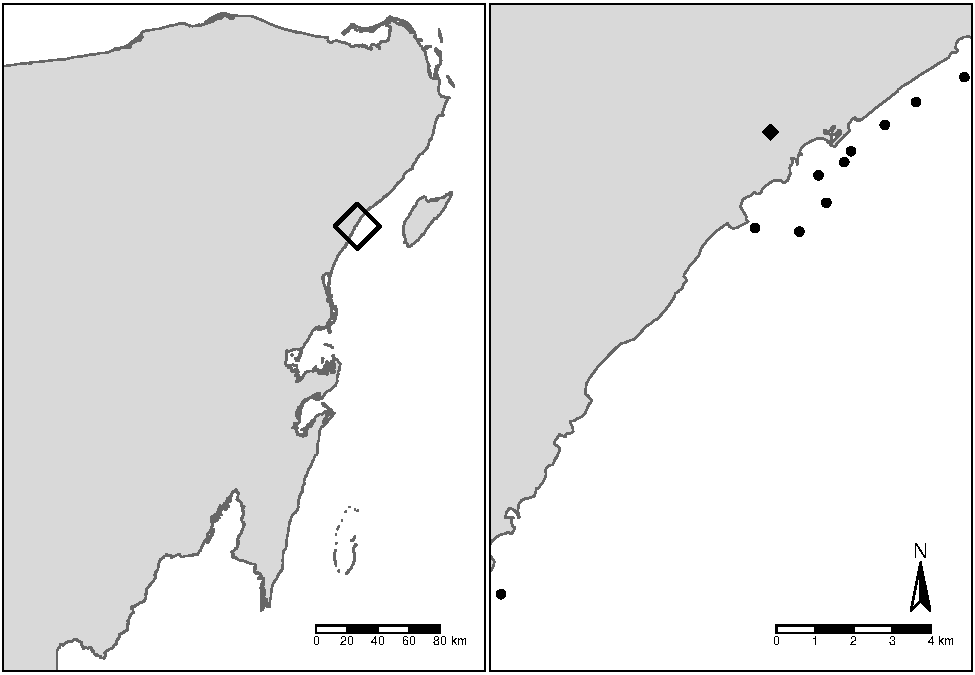
\includegraphics{Manuscript_files/figure-latex/unnamed-chunk-6-1.pdf}
\caption{Map of the study area. The black inset on the left (Yucatan
Peninsula) indicates the location where study sites are distributed. On
the right, circular markers indicate sampling sites and the black
romboid indicates location of Puerto Aventuras, Mexico.}
\end{figure}

\clearpage

\begin{figure}[htbp]
\centering
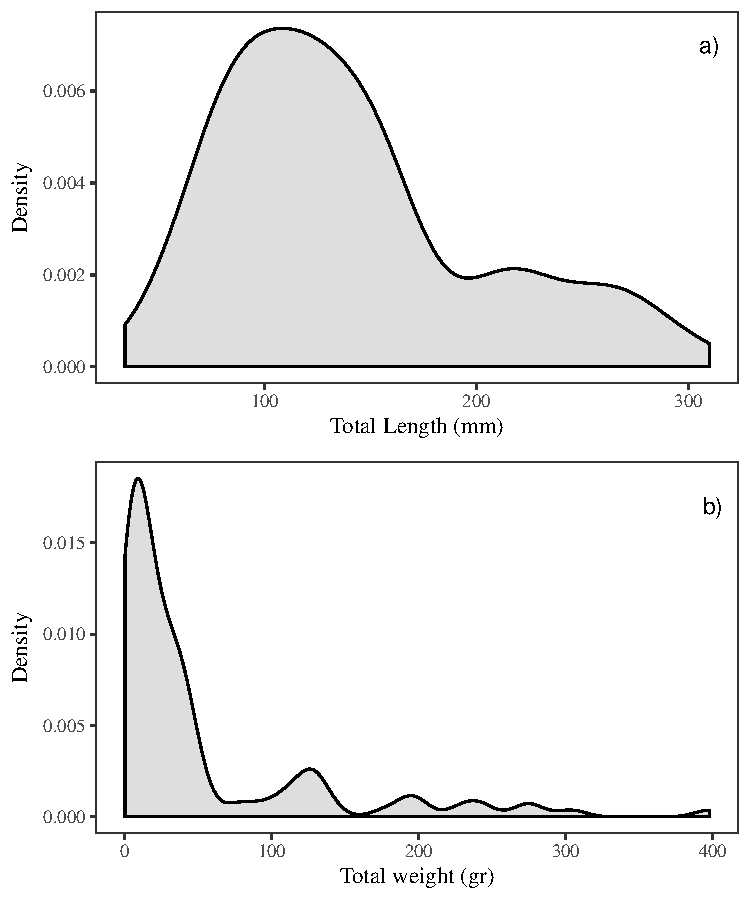
\includegraphics{Manuscript_files/figure-latex/unnamed-chunk-7-1.pdf}
\caption{Kernell density plots for a) Total length (mm) and b) Total
weight (gr) for 109 lionfish sampled in the central Mexican Caribbean.}
\end{figure}

\clearpage

\begin{figure}[htbp]
\centering
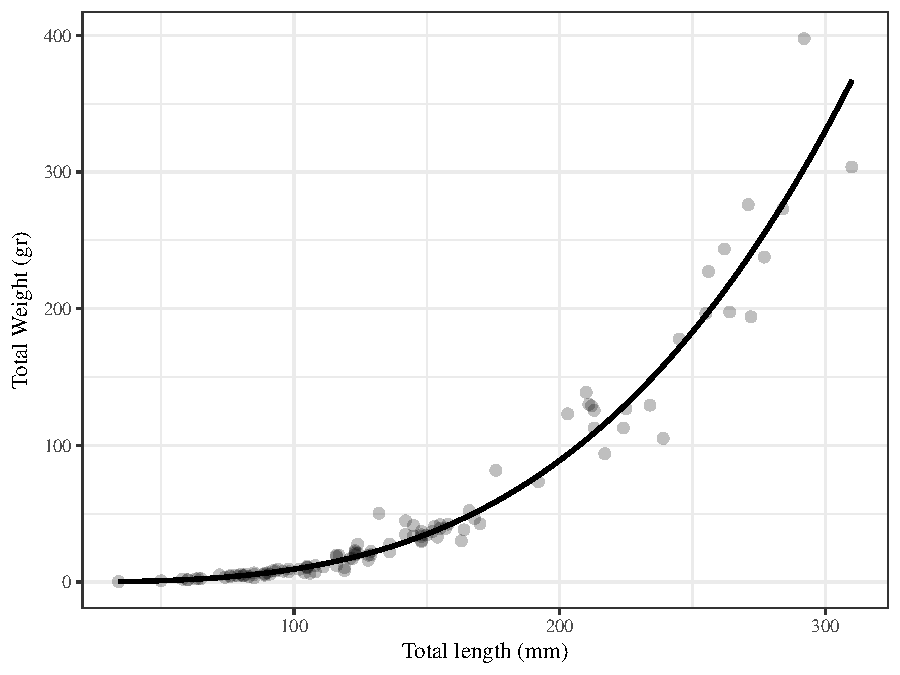
\includegraphics{Manuscript_files/figure-latex/unnamed-chunk-8-1.pdf}
\caption{Length-weight relationship for 109 lionfish sampled in the
central Mexican Caribbean. Points indicate samples, solid line indicates
curve of best fit.}
\end{figure}

\clearpage

\begin{figure}[htbp]
\centering
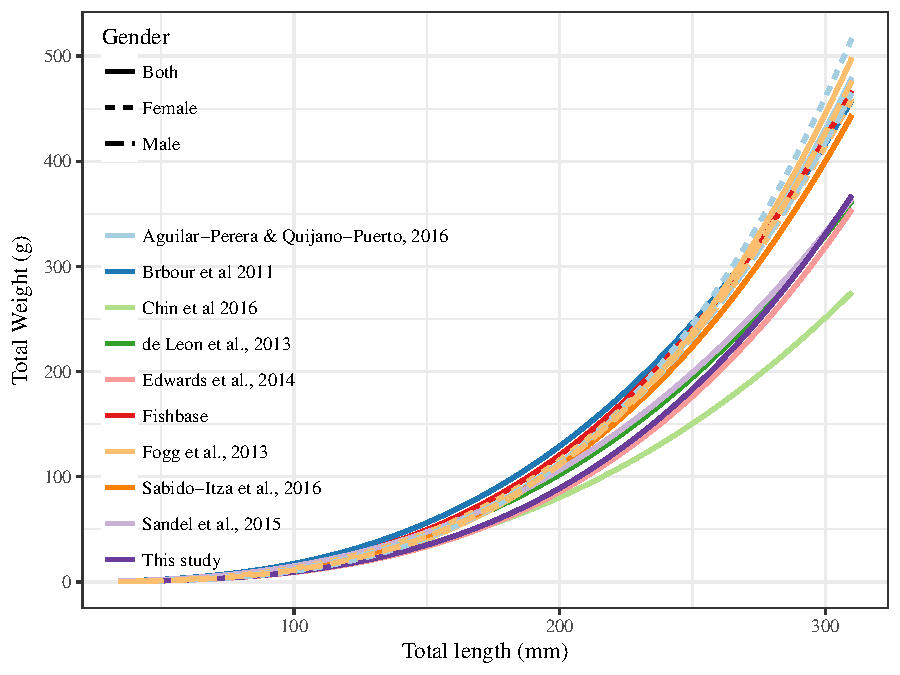
\includegraphics{Manuscript_files/figure-latex/unnamed-chunk-9-1.pdf}
\caption{Length-weight relationships (n = 14) for eight studies, this
study, and Fishbase. Colors indicate studies from which the parameters
were extracted. Solid lines indicate that the fit was performed for
males and females pooled together. Dotted lines indicate that the
regression was performed on females, and dashed lines indicate it was
performed for males.}
\end{figure}

\clearpage

\begin{figure}[htbp]
\centering
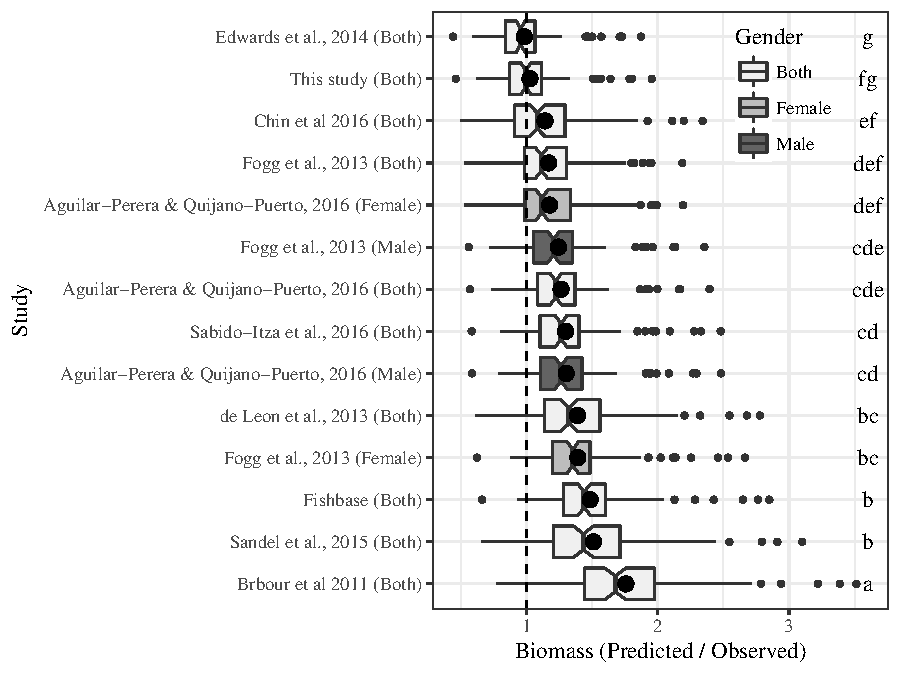
\includegraphics{Manuscript_files/figure-latex/unnamed-chunk-10-1.pdf}
\caption{. Box and whiskers plot showing the distribution of predicted
to observed biomass ratios for 14 pairs of allometric parameters. Lines
indicate median values, circles indicate mean values, notches represent
95\% confidence intervals arround the median, lower and upper hinges
correspond to the first and third quartiles, whiskers extend to the
largest and lowes values within 1.5 inter-quartile range of the hinge,
small points represent outliers further away than the whiskers. Like
letters indicate values that do not differ significantly (Tukey's HSD; p
\textless{} 0.05).}
\end{figure}


\end{document}
